\renewcommand{\thechapter}{\Roman{chapter}}
\chapter{Review of Related Literature}
\renewcommand{\thechapter}{\arabic{chapter}}
\label{ch:rrl}
\thispagestyle{empty}

Enhancing post-harvest processing and storage technology is essential meeting increasing global demand and minimizing waste. Improved technology ensures efficient supply chains and reduces losses due to spoilage, damage, or inefficient methods. Moreover, advanced monitoring and management techniques not only enhance production but also contribute to safety standards \citep{Kumar2017-jl,Joni2022}.

In this chapter, various relate topic were reviewed and discussed. Different methods, technologies and implementation were also introduced and examined.

\section{Overview of Existing Methods, Techniques and Technologies Used for Volume Measurement}

%In this chapter, the researcher discussed the general idea of the volume estimation and filtering method and its several related studies. The chapter also presented some published and unpublished methods and technologies used for measuring the level and volume of the materials inside the silo (or sometimes called bin).
According to \citet{turner2016}, the determination of grain volume in a bin depends on variables like bin diameter and corresponding level height of grain. Different surface condition assessment, however, is subjective and subject to a number of variables, such as operator experience, visibility, lighting, and ambient circumstances. Various strategies can be used to improve volume estimate; standard angles of repose for various grain types are provided in the literature.

Traditional level measurements are already used and studied in different industries such as weight and cable methods, ultrasonic, Guided Ware Radar (GWR), and Thru-air Radar (TAR) which has their own advantage and disadvantages. Ultrasonic and laser technologies are excellent in providing accurate and detailed measurement of level. However, these technologies are problematic when in terms of dusty environment \citep{duysak2020}. Additionally, Various tools and methods have been developed to measure stored raw materials volume inside an industrial storage silos or bins, employing sensors like contact level indicators (e.g., tilt switches, pressure diaphragms, rotary paddles) and non-contact indicators (e.g., stereovision, radar, ultrasound, lasers). Contact sensors offer cost-effective, dust-resistant point measurements but lack surface detail. Non-contact sensors can map grain surfaces accurately but require permanent mounting, are relatively expensive, and are susceptible to dust interference. However, conventional volumetric measurement method using weighted fiberglass tape is still being used providing only a single data point which leads to inaccuracy and error-prone volume measurement due to uneven materials  surface topology \citep{turner2016,turner2017}.

New methods and technologies have been trying to incorporate in industrial settings to enhance the measurement methods such as using Microwaves Radar \citep{vogt2017}, Horn Antennas-based \citep{duysak2020, yigit2015}, Load Cell, Ultrasonic, Laser-based \citep{geuvara2020}, and Temperature-based sensor \citep{rhee2021}.

\section{Point Cloud Acquisition Devices}
\label{rrl:sec:3D Point Cloud acquisition}
The recent advancements in spatial acquisition technologies such as 3D laser scanning, photogrammetry, videogrammetry, RGB-D camera, and stereo camera have resulted in the formation of point clouds that may contain millions, billions, or trillions of points \citep{jaboyedoff2012}. Various 3-dimensional scanning technology produces data that are formatted as point cloud, typically these point cloud data acquired using laser or image scanner. These gathered data can be managed to ease the measurement and visualization of an object or environment \citep{chua2017}. Point cloud data are processed to generate desired output on the specific application. Over the past 20 years, the advent of high-quality 3D point cloud acquisition changes the perspective of robotics. Moreover, 3D scanning through various technologies enable the possibility of less contact for physical measurement that eliminate the traditional approach that involves time and effort. These technologies vary in size, functionality, and cost, ranging from affordable options to more complex and expensive ones \citep{rusu2011}.


\subsection{Light Detection and Ranging (LiDAR)}
\label{rrl:subsec:Light Detection and Ranging}
LiDAR, a remote sensing technology, employs laser light to create precise 2D or 3D models of objects or environments. Apart from Time-of-Flight (ToF) and triangulation, which measures distances based on the angle and timing of laser pulses, LiDAR systems utilize other techniques such as amplitude modulation and frequency modulation. These techniques vary in how they measure distances and capture data. By integrating data from multiple laser pulses, LiDAR generates a comprehensive point cloud that accurately represents the shape and structure of the objects within the environment, Figure \ref{fig:Typical LiDAR System} shows the block diagram of a typical LiDAR system. LiDAR technology have been used in industrial settings. In the context of LiDAR scanning, individual point cloud scans are acquired and processed for a specific area. These point clouds are then merged and blended together to generate a complete point cloud of the desired area, which can be utilized for distance and measurement calculations \citep{jaboyedoff2012, raj2020}.

\begin{figure}[H]
	\centering
	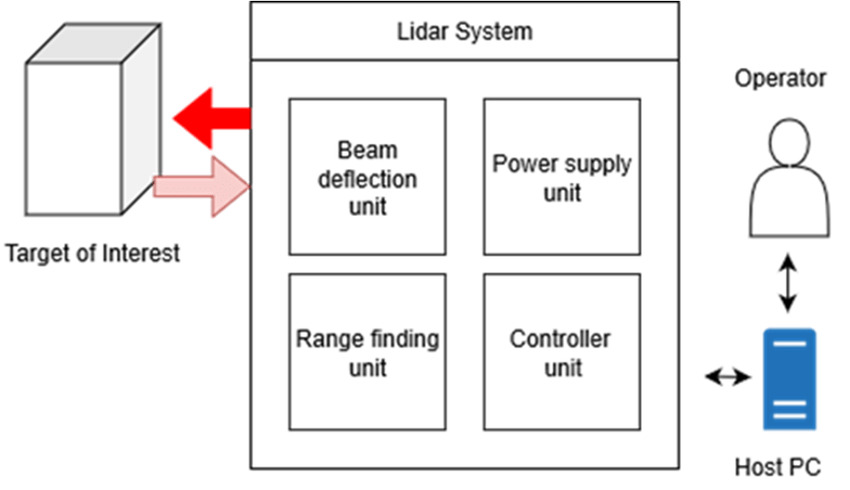
\includegraphics[width=0.9\textwidth]{Figures/Block-diagram-of-light-detection-and-ranging-LiDAR-system} % second figure itself
	\caption{Typical LiDAR System}
	\label{fig:Typical LiDAR System}
\end{figure}

A 360-degree scan of a LiDAR is generally obtained as shown in figure \ref{fig:360-dgree-lidar-scan} to produce a 2D map, a typical scan using the robot's top-mounted 2D LIDAR. The axis of the rotating LIDAR sensor is shown as a red line. The border of the surrounding obstacles is indicated in blue \citep{sarker2020}.

\begin{figure}[H]
	\centering
	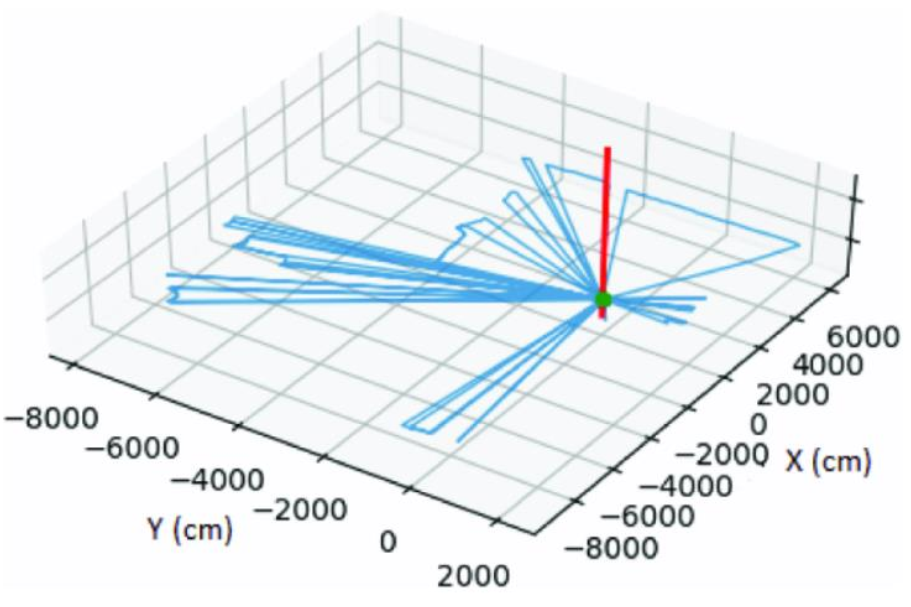
\includegraphics[width=0.9\textwidth]{Figures/360-degree-lidar-scan.png} % first figure itself
	\caption{360-degree scan of 2D LiDAR}
	\label{fig:360-dgree-lidar-scan}
\end{figure}

\subsection{Rotating 2D LiDAR Scanner into a 3D Point Cloud Scanner: Mechanisms and Techniques}
A 2D LiDAR scanner, typically used for horizontal plane scanning, can be transformed into a 3D point cloud scanner with the addition of extra components and processing techniques. One common method involves incorporating a rotating mechanism, such as a pan-tilt unit (PTU), to the 2D LiDAR. As the LiDAR rotates, it collects data points at various angles, generating a series of 2D scans. These scans are then combined and processed using algorithms to reconstruct a 3D representation of the surroundings. Integrating the 2D LiDAR device with electric motors into various configurations enables the acquisition of 3D scans. Figure \ref{fig:four_different_configurations} illustrates four such configurations: pitching, rolling, yawing, and top yawing scans \citep{raj2020}.

\begin{figure}[H]
	\centering
	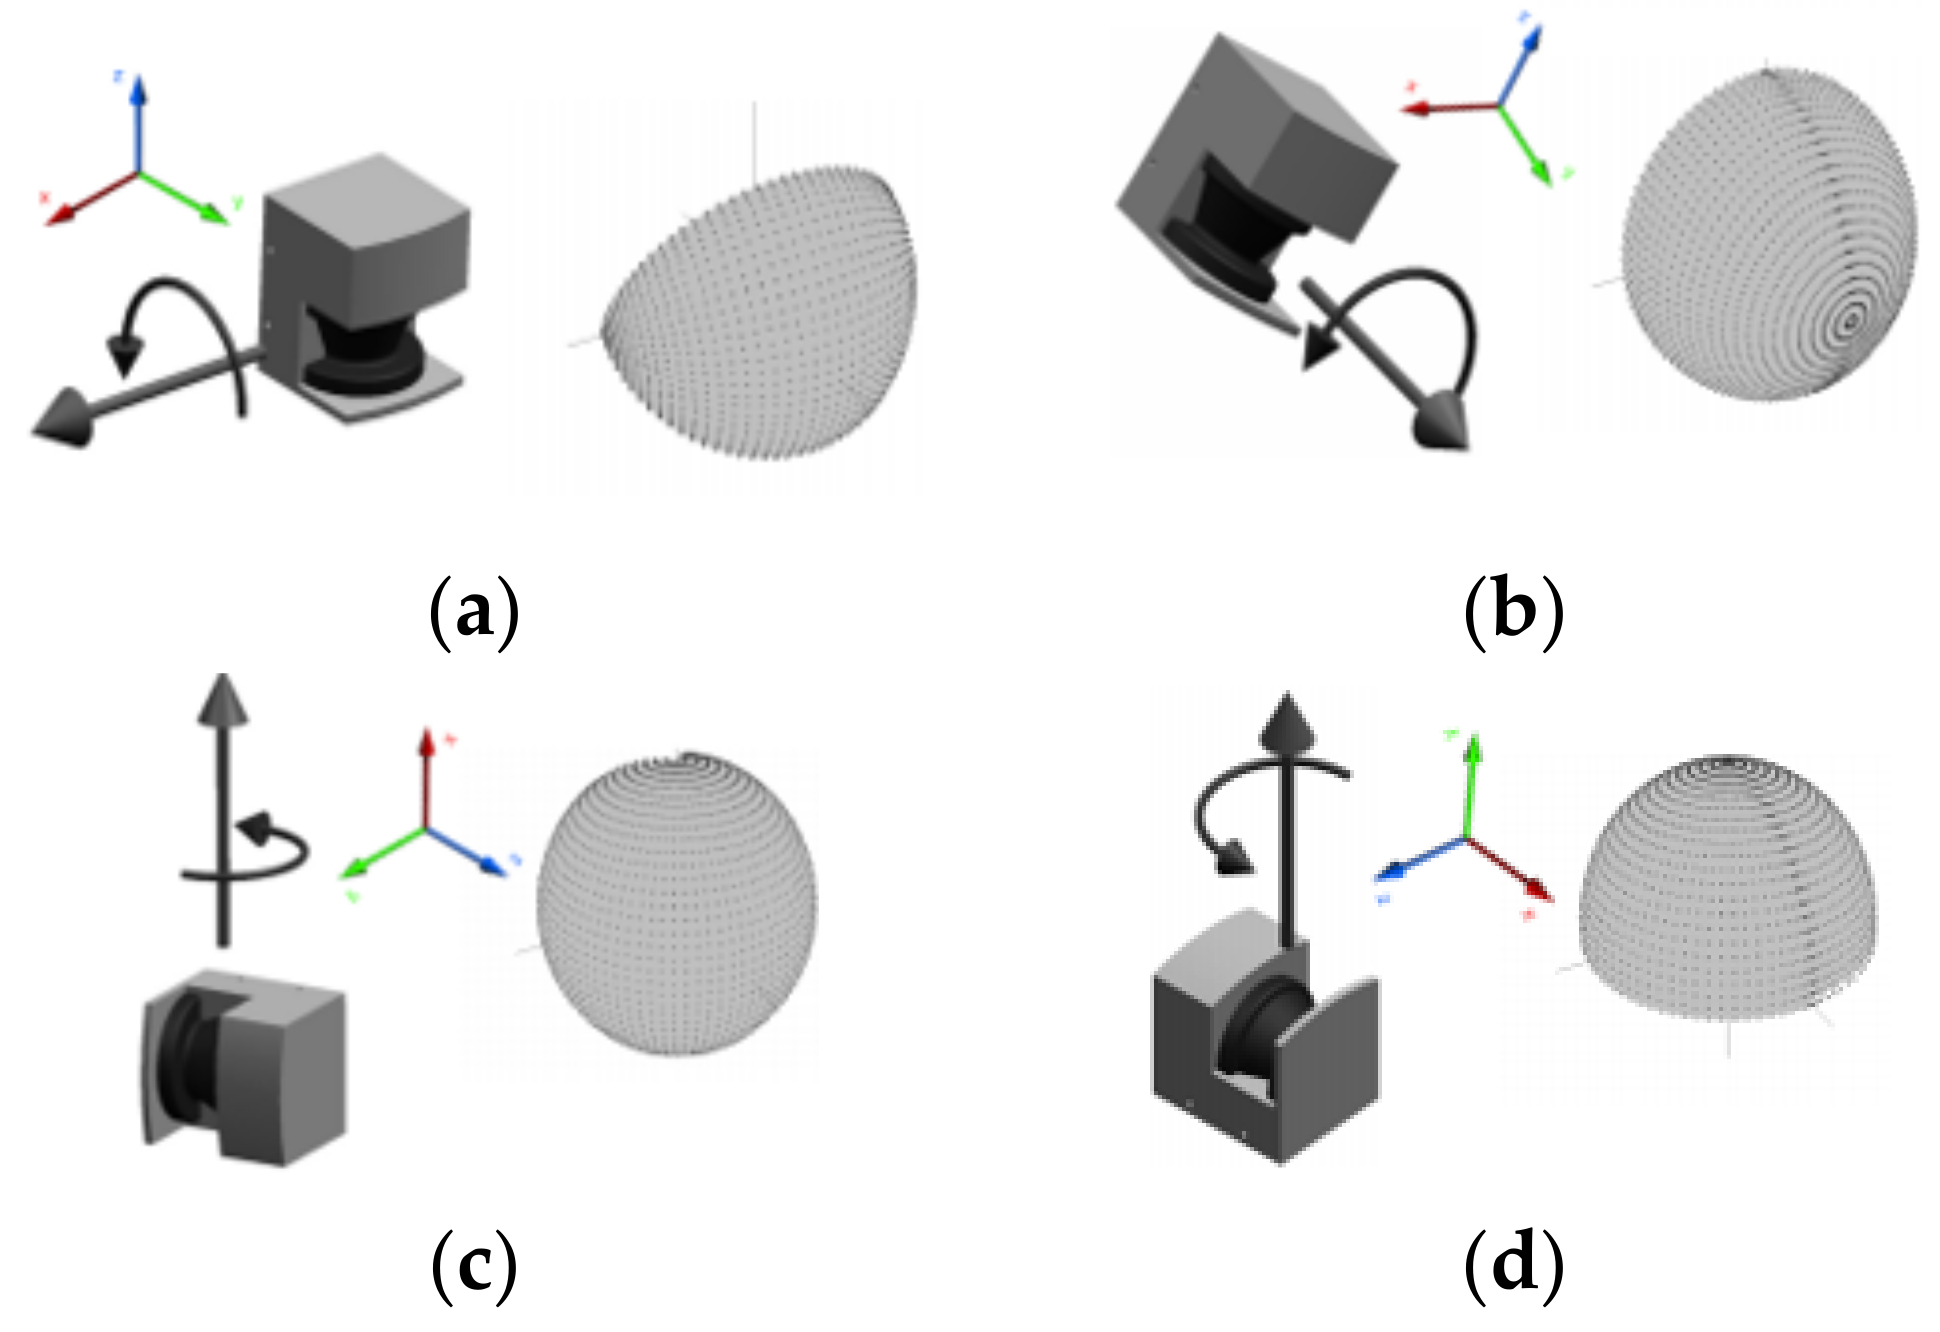
\includegraphics[width=0.9\textwidth]{Figures/tilting} % include your image file here
	\caption{Four different configurations for rotating: (a) pitching scan, (b) rolling scan, (c) yawing scan, (d) top yawing scan}
	\label{fig:four_different_configurations}
	\medskip
	\normalsize Source: \citep{raj2020}
\end{figure}

% \begin{figure}[H]
% 	\centering
% 	\begin{minipage}{0.5\textwidth}
% 		\centering
% 		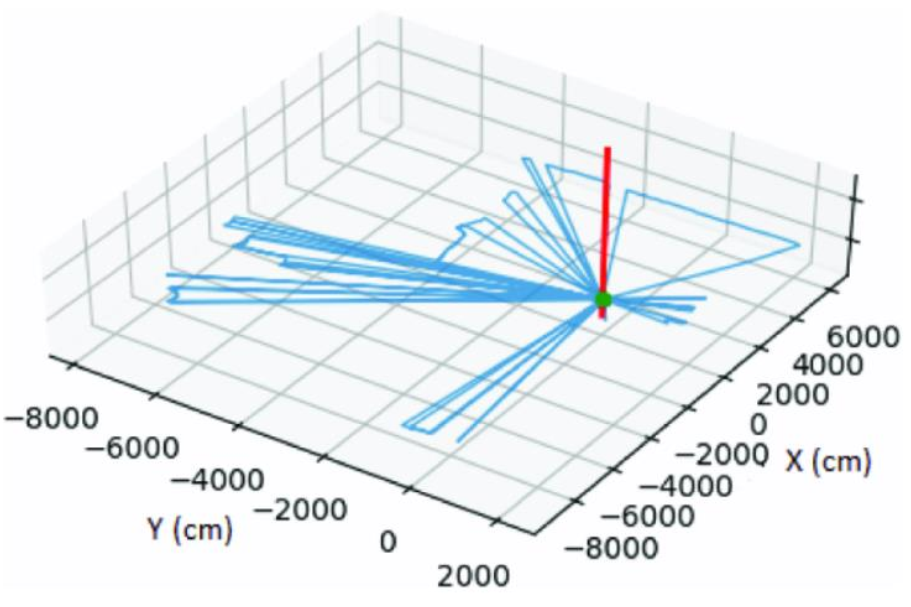
\includegraphics[width=0.9\textwidth]{Figures/360-degree-lidar-scan.png} % first figure itself
% 		\caption{360-degree scan of 2D LiDAR}
% 		\label{fig:360-dgree-lidar-scan}
% 	\end{minipage}\hfill
% 	\begin{minipage}{0.5\textwidth}
% 		\centering
% 		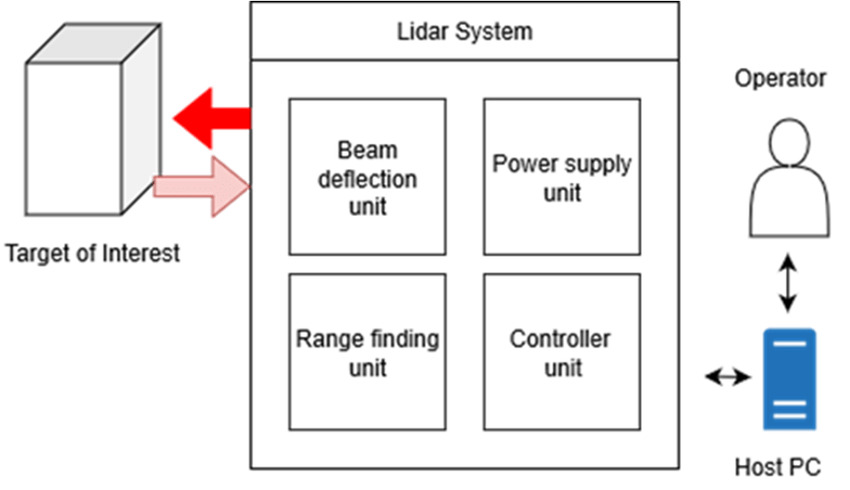
\includegraphics[width=0.9\textwidth]{Figures/Block-diagram-of-light-detection-and-ranging-LiDAR-system} % second figure itself
% 		\caption{Typical LiDAR System}
% 		\label{fig:Typical LiDAR System}
% 	\end{minipage}
% \end{figure}

\citet{kang2018} utilized a 2D low-cost off-the-shelf LiDAR to reconstruct complex 3D model by integrating an external rotary for additional dimension. The experimental test achieved to evaluate 3D reconstruction by concluding that using a low-cost 2D LiDAR sensors can  perform 3D point cloud acquisition but increase either the complexity of its hardware or software.

A stepper motor was used in the study conducted by \citet{yuan2021} and \citet{kang2018} to rotate a 2D LiDAR. However, in the study conducted by \citet{yuan2021}, the rotating 2D LiDAR with initial motor shaft position defined using a combination of photoelectric switches and shading sheets, to create a 3D point cloud representation of the environment. The main objective of the study was to minimize the cost by utilizing stepper motor. Intensive calibration was conducted to correct the error of the system due to lack of the absolute angle position of the motor, thus, the study focus on calibrating the system by synchronizing the 2D LiDAR with the stepper motor.

In a previous study by \citet{clar2022}, a servo motor was employed to rotate a 2D LiDAR, with calibration performed to synchronize the LiDAR's movement. However, the system in that study relied on a laptop and microcontroller for operation. While adequate for small-scale and laboratory experimental testing, this setup posed challenges for larger-scale deployment due to its size, weight, and power demands. Consequently, there arose a need for a more compact and portable solution to address these limitations.

The primary problem with calibration and synchronization between a 2D lidar and a servo arises from the lack of an absolute angle reference for the servo. Unlike encoders or sensors that provide precise angular measurements, servos typically lack absolute positioning capabilities. Although rotating 2D LiDAR can never replace commercial 3D LiDAR with several reasons, however, rotating 2D LiDAR can be partially used and installed with in terms of static and nonmoving environment \citep{bi2021}.

\section{Volume Measurement Using 3D Point Cloud Data}

Utilizing the latest advances in volume measurement with 3D point cloud data is an innovative method that precisely determines the volume of spaces or objects in a three-dimensional environment. This technique makes precise and thorough volumetric analysis possible by using point cloud data, which frequently consists of millions of points in 3D space. The concepts, procedures, and uses of volume measurement with 3D point cloud data will be covered in explain in this section, along with examples of its relevance in various domains \citep{zhi2016,meng2023}.

\subsection{Frameworks for Point Cloud Processing, Visualization, and Mapping}
Various point cloud processing and mapping frameworks are widely available to lessen the complexity of handling raw point cloud data, such as, Robotic Operating System (ROS), Point Cloud Library (PCL), Open3D, MeshLab, etc. Most of this framework can be used in many different fields such as virtual reality, construction, industry, and surveying.

The PCL has a built-in visualization library that uses Visualization ToolKit (VTK) as its foundation. VTK is a versatile platform that can render 3D point clouds and surfaces, and supports visualizing tensors, textures, and volumetric methods. The PCL Visualization library aims to merge PCL with VTK by providing a complete visualization layer for n-D point cloud structures. Its main goal is to allow for rapid prototyping and visualization of algorithm results on high-dimensional data \citep{rusu2011}.

\citet{ocando2017} take advantage of using ROS framework to map the 3D point cloud data, as the framework allows to interlink programs that is written in different languages. The study successfully addressed the problematic tasks of Simultaneous Localization and Mapping (SLAM) and 3D Octomapping via single sensor. \citet{clar2022} also utilizes ROS framework and PCL to filter, convert and measure the volume of the gathered point cloud data.

\subsection{Techniques and Methods for Volume Estimation Using Computational Geometry}

Point clouds in 3D are highly valuable as they contain crucial information on the shape, size, area, and volume of objects. Various industries, including agriculture and fisheries, have effectively utilized volume estimating methods based on point clouds \citep{geuvara2020}.

Due to a better portrayal of the region encompassed in the group of points, the Delaunay triangulation and voxelization procedures outperform in estimating the outcomes. These strategies, however, have a greater computational cost because of their accuracy \citep{chee2015}. To estimate volume, methods such as Delaunay triangulation and voxelization are used. It is important to consider both accuracy and computing costs when using these methods. Height grids are faster for computing height discrepancies, but accuracy depends on precise point acquisition \citep{bewley2011, duff2000}.

The Delaunay triangulation-based technique for volume computation, known as Delaunay triangulation-driven volume calculation (DTVC), differs from traditional approaches which computes the volume during the triangulation process rather than preserving Delaunay triangles. This method reduces both memory usage and processing time. Experimental findings demonstrate that DTVC achieves a satisfactory trade-off between precision and efficiency \citep{liuY2021}.

In computer graphics, a voxel is an image that depicts a specific region that has been partitioned into a grid of cubes that are all the same size and uniformly spaced \citep{putman2018}.

The Convex Hull is another method that is popular technique for measuring volume from 3D point cloud points (see figure \ref{fig:convex hull}). The computational geometry community has extensively studied the convex hull problem, as evidenced by the works of \citet{kim2002}, \citet{graham1983}, and \citet{maus1984}. Qhull is a commonly used algorithm to compute the convex hull, employing the Voronoi diagram, the Delaunay triangulation, furthest-site Voronoi diagram, the furthest-site Delauney triangulation, and the half-space intersection around a point. The software program allows the creation of high-dimensional objects, and the Quickhull algorithm, written in C, is used to compute the convex hull, which solves round-off errors in floating-point arithmetic. The program is capable of calculating volumes, surface areas, and convex hull approximations.

\begin{figure}[H]
	\centering
	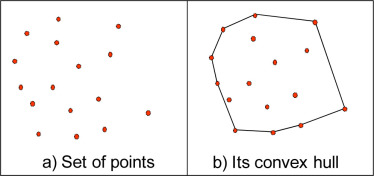
\includegraphics[width=0.8\textwidth]{Figures/convex hull.jpg}
	\caption{Convex Hull}
	\label{fig:convex hull}
\end{figure}

Table \ref{tab:Point Cloud Volume of Different Objects} shows the percentage error analysis from the computed volume of different model point cloud objects in the study of \citet{chang2017}, which shows that in order to estimate the volume of a shape represented by a point cloud, the area of each slice of the shape is calculated by finding the difference between the top and bottom curves of the slice. The total volume of the shape is then calculated by integrating the areas of all the slices using an integration interval equal to the length of the point cloud.

\begin{table}[H]
	\caption{Point Cloud Volume of Different Model}
	\label{tab:Point Cloud Volume of Different Objects}
	\centering
	\begin{tabular}{l c c r}
		\toprule
		% First row
		\textbf{Objects} & \textbf{True Value (\si{mm^3})} & \textbf{Estimated Value (\si{mm^3})} & \textbf{Error} (\%) \\
		\midrule
		% Second row
		Cube             & 1 000 000                       & 1 000 000                            & 0                   \\

		% Third row
		Cylinder         & 125.664                         & 125.061                              & 0.479               \\

		% Fourth row
		Sphere           & 4 188 90.2                      & 4 178 966.87                         & 0.234               \\

		% Fifth row
		Triangle Prism   & 17.321                          & 17.399                               & 0.45                \\
		\bottomrule
	\end{tabular}
\end{table}

The study conducted by \citet{jeong2018} introduces a newly developed explicit hybrid numerical methodology for 3D volume reconstruction from unorganized point clouds, which is based on a modified Allen-Cahn equation and a 3D binary picture segmentation method. The technique has demonstrated potential in a variety of practical applications, including 3D model printing from dispersed scanned data. The computational findings show that the suggested approach for reconstructing 3D volume from point clouds is very efficient and resilient.

\section{Robot Web Tools Application for ROS Remote Monitoring}

The integration of Robot Web Tools (RWT) with ROS has garnered significant attention in recent years due to its potential to revolutionize real-time robotics applications. By leveraging web technologies and cloud computing infrastructure, developers aim to create intuitive interfaces for controlling and monitoring robots remotely. Central to the capabilities of RWT is its efficient messaging mechanism, which enables real-time interaction between web-based interfaces and ROS-enabled robots. By leveraging technologies such as roslibjs and rosbridge, RWT facilitates the seamless exchange of data, including sensor readings, point clouds, and control commands. This efficient messaging paradigm forms the backbone of RWT's ability to provide responsive and interactive interfaces for controlling and monitoring robotic systems.

Several studies have explored the capabilities of RWT in enabling real-time interaction with ROS-enabled robots. For instance, in a study by \citet{qureshi2016poster}, the development of a disaster management application is showcased, wherein Robot Web Tools (RWT) is utilized for seamless communication with ROS nodes. This integration enables an efficient response to emergencies by facilitating real-time interaction and control of robots remotely.

Furthermore, \citet{lim2019cloud} explored the integration of ROS with cloud computing infrastructure to offload computationally intensive tasks and enhance scalability. They utilized RWT to develop web-based visualization tools for analyzing sensor data in real-time, showcasing its versatility in cloud robotics applications.

% The development of a measuring system for accurately defining grain surfaces led to the creation of a bin measurement system utilizing a laser distance meter, as described by \citet{turner2017}. According to the findings of the study, sophisticated data processing techniques were developed to simulate complicated grain surfaces, making it possible to estimate grain volume using the generated surface and bin geometry. However, the requirement for manual post-processing and visual examination restricted the automation of data processing. Moreover, the system's efficacy relied on a clear view of the entire grain surface \citep{turner2017}.

% \section{Point Cloud Processing}
% \label{rrl:sec:Point Cloud Processing}
% Recent advancements in 3D reconstruction and visualization based on point cloud data have led to rapid development in various fields due to the rich data information and detailed real-world representation of objects or environments. Consequently, this massive data, including enormous kinds of noise, is overwhelmingly tedious to manage \citep{li2020}.

% In the study conducted by \citet{wang2020}, when point cloud data are involved in construction applications, different point cloud data processing procedures are crucial to achieving desired outputs. Figure \ref{fig:data-processing} shows the common procedures for the raw point cloud data in a construction setting \citep{wang2020}.

% \begin{figure}[H]
% 	\centering
% 	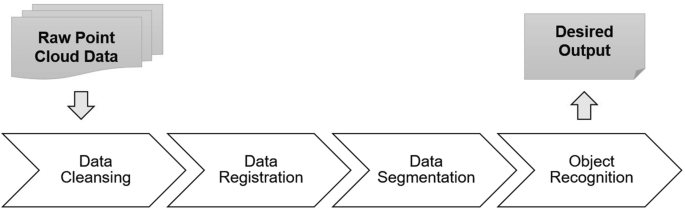
\includegraphics[width=0.9\textwidth]{data-processing}
% 	\caption{Typical processing procedures of point cloud data}
% 	\label{fig:data-processing}
% \end{figure}

% \citet{stanislas2021} divided the point cloud processing into four-step processes, figure \ref{fig:The-four-stages-of-the-point-cloud-classification-process} illustrates the structure of the authors, the point cloud output of the method is the same point cloud that was inputted before the classification took place. The method involves feature computing, data formatting, network prediction, and post-processing.

% \begin{figure}[H]
% 	\centering
% 	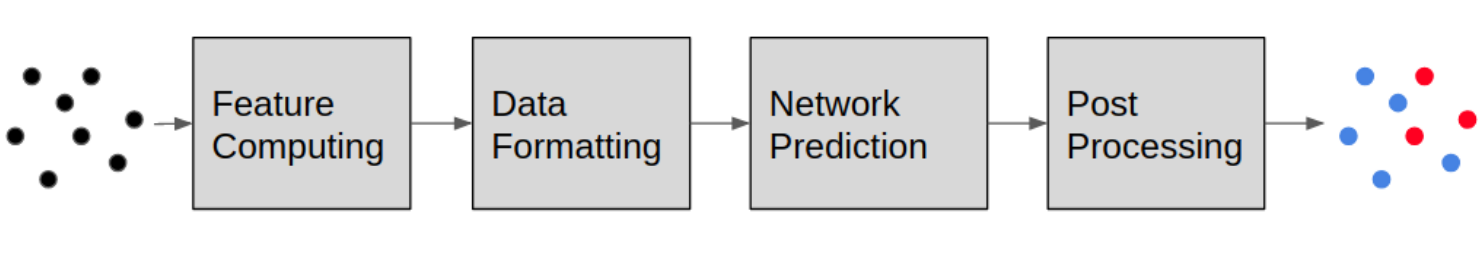
\includegraphics[width=\textwidth]{Figures/four-stage-of-pc-classification-process.png}
% 	\caption{The four stages of the point cloud classification process}
% 	\label{fig:The-four-stages-of-the-point-cloud-classification-process}
% \end{figure}

% \subsection{Outlier Point Cloud Processing}
% \label{sub:Point Cloud Processing}
% Processing of point cloud data by filtering is intensively exposed in research with a wide variety of applications. Cleaning of raw 3D point clouds is commonly the first step for most geometry processing, it involves removing the outliers (e.g., dust, snow, fog, etc.) after classifying the dust and non-dust (inliers) point cloud, smoothing the remaining data, and then reconstructing the surface into a three-dimensional representation \citep{rakotosaona2020}. Artificial Intelligence techniques such as Machine Learning (ML) and Deep Learning (DL) are widely used in classifying point cloud dust and non-dust data to remove noise.

% For instance, \citet{stanislas2018} detected dusty regions in point cloud data by using machine learning techniques as well as specialized neural networks. The 3D map was transformed into 3D occupancy grids in this investigation, and the occupied voxels were utilized to train classifiers based on machine learning to extract significant information, figure \ref{fig:pcl seg} shows the result of the study.

% \begin{figure}[H]
% 	\centering
% 	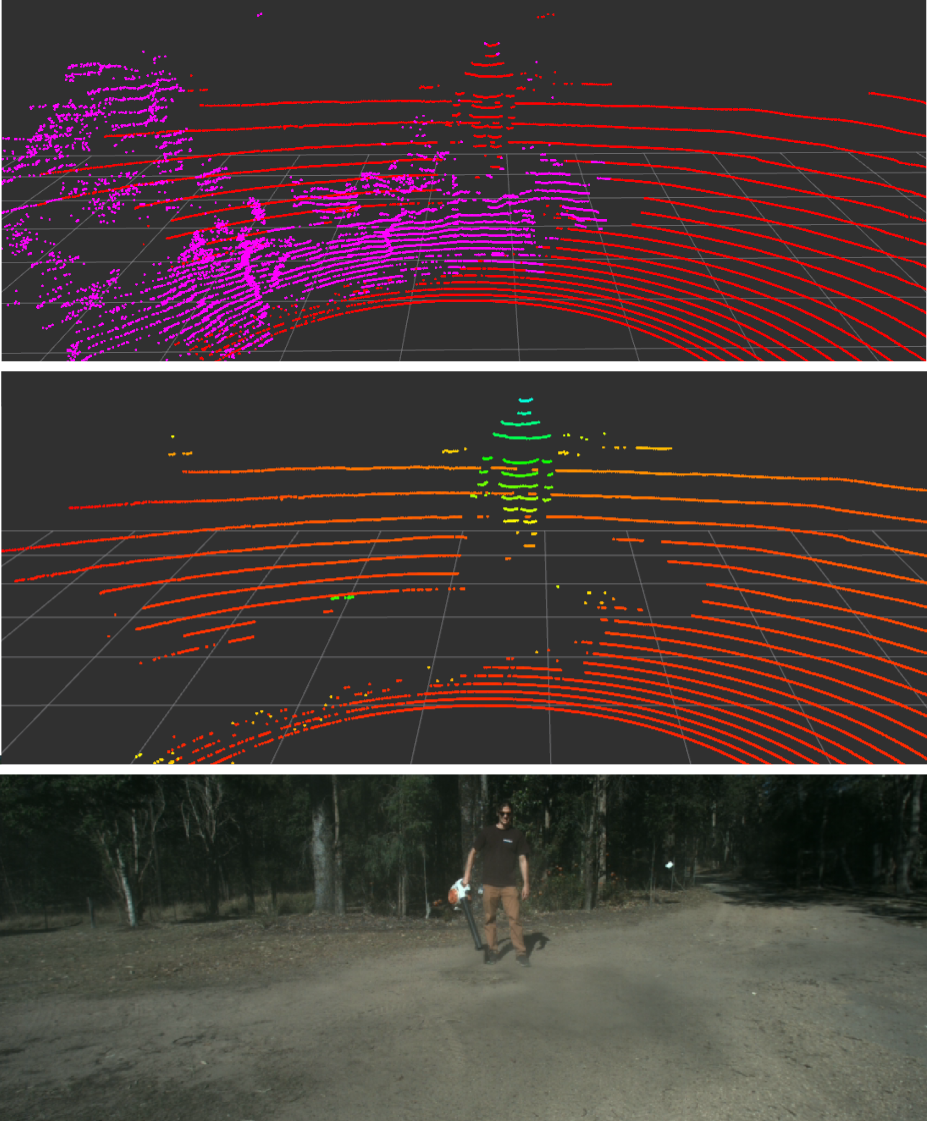
\includegraphics[width=0.7\textwidth]{pcl_seg}
% 	\caption{Top: Detection of airborne dust particle in a LiDAR point cloud, purple is Particle and red is Non-particle. Middle: Removal of detected dust particles from point cloud for robust perception, the color is mapped to the vertical axis (red is low, green is high). Bottom: Image depicting the scene.}
% 	\label{fig:pcl seg}
% \end{figure}

% The same voxel-based approach was also used in the study of \citet{shamsudin2016} for the classification of fog. The method involved using geometrical features and intensity as inputs for the support vector machine (SVM) and k-nearest neighbors (KNN) algorithms to classify fog.

% Both point- and voxel-based categorization were taken into account in study by \citet{stanislas2021}. They experimented with various classifier input features to determine the most effective one for dust removal in order to boost performance. These characteristics include geometry, intensity, and multi-echo data from the LiDAR sensor. With point-based deep learning techniques, geometry, and multi-echo features proved to be the most useful features, while voxel-based deep learning techniques benefited from the addition of intensity information to these features.

% To simplify the point cloud models and reduce the noise in point cloud data, \citet{zhu2020} employed the point-based simplification and guided filter. The guided filter was employed to filter the noisy point cloud model and generate the filtered image. The surface-based filtering group employs the filtering algorithm.

% \citet{ramiya2017} set a threshold by measuring the distance between every point and the mean surface. They assigned a weight to each point based on its distance from the interpolated mean surface.

% \citet{heinzler2020} used a large point cloud data set for CNN-based approach segmentation in controlled adverse weather effects. The approach takes a global understanding of the scene to estimate the validity of individual point measurements, rather than analyzing local spatial statistics as in previous approaches, it also proposes data augmentation technique that reduces the necessity for annotated ground truth data.

% The multi-echos and intensity data features of LiDAR point cloud are utilized in various studies. \citet{afzalaghaeinaeini2021} used low-intensity outlier removal (LIOR) filtering for de-dusting method. The method is composed of two procedures: First, dust particles based on point cloud usually have a lower intensity compared to non-dust point cloud, point cloud with an intensity lower than the set threshold are removed. Second,  the study successfully filtered the point cloud data and removed the dust from the original point cloud data.

% Intensity-based filter was also utilized by \citet{park2020} for removal of snow in point cloud data. The study concluded that this method overcomes the disadvantages of LiDAR sensor compared to other conventional filtering methods.

% \subsection{3D Space Point Cloud Mapping}

% In todays generation, various point cloud processing and mapping frameworks are widely available to lessen the complexity of handling raw point cloud data, such as, Robotic Operating System (ROS), Point Cloud Library (PCL), Open3D, MeshLab, etc. Most of this framework can be used in many different fields such as virtual reality, construction, industry, and surveying.

% The PCL has a built-in visualization library that uses Visualization ToolKit (VTK) as its foundation. VTK is a versatile platform that can render 3D point clouds and surfaces, and supports visualizing tensors, textures, and volumetric methods. The PCL Visualization library aims to merge PCL with VTK by providing a complete visualization layer for n-D point cloud structures. Its main goal is to allow for rapid prototyping and visualization of algorithm results on high-dimensional data \citep{rusu2011}.

% \citet{ocando2017} take advantage of using ROS framework to map the 3D point cloud data, as the framework allows to interlink programs that is written in different languages. The study successfully addressed the problematic tasks of Simultaneous Localization and Mapping (SLAM) and 3D Octomapping via single sensor.

% \section{Volume Estimation}
% \label{rrl:sec:Industrial Volume Measurement}
% Typically in an agriculture and food company setting, calculating the volume of a storage bin involves determining both the storage geometry and the distance between the grain surface and the eave. Traditionally, a fiberglass tape measure with weights is used to calculate the distance between the surface of the grain and the top of the bin. Correction factors are applied to the measurement to account for any irregularities in the surface of the grain, such as when the surface is uneven or when there is a cone-shaped pile \citep{turner2016}. These correction factors are usually simple to apply when the surface is relatively flat and equal in height. Moreover, these traditional approaches necessitate such effort and involved the employees to be at the top of the bin during the estimation. New methods and technologies have been trying to incorporate in industrial settings to eliminate these traditional methods such as using Microwaves Radar \citep{vogt2017}, Horn Antennas-based \citep{duysak2020, yigit2015}, Load Cell, Ultrasonic, Laser-based \citep{geuvara2020}, and Temperature-based sensor \citep{rhee2021}. Each of this technology has their own advantage and disadvantages, however, laser-based sensor (e.g. LiDAR) shows an interesting capabilities and features especially in acquiring three-dimensional point cloud data that can be used for geometric computation and for 3D object representation.

% Point clouds in 3D are highly valuable as they contain crucial information on the shape, size, area, and volume of objects. Various industries, including agriculture and fisheries, have effectively utilized volume estimating methods based on point clouds \citep{geuvara2020}.

% In computer graphics, a voxel is an image that depicts a specific region that has been partitioned into a grid of cubes that are all the same size and uniformly spaced \citep{putman2018}.

% Due to a better portrayal of the region encompassed in the group of points, the Delaunay triangulation and voxelization procedures outperform in estimating the outcomes. These strategies, however, have a greater computational cost because of their accuracy \citep{chee2015}. To estimate volume, methods such as Delaunay triangulation and voxelization are used. It is important to consider both accuracy and computing costs when using these methods. Height grids are faster for computing height discrepancies, but accuracy depends on precise point acquisition \citep{bewley2011, duff2000}.

% The Delaunay triangulation-based technique for volume computation, known as Delaunay triangulation-driven volume calculation (DTVC), differs from traditional approaches which computes the volume during the triangulation process rather than preserving Delaunay triangles. This method reduces both memory usage and processing time. Experimental findings demonstrate that DTVC achieves a satisfactory trade-off between precision and efficiency \citep{liuY2021}.

% Table \ref{tab:Point Cloud Volume of Different Objects} shows the percentage error analysis from the computed volume of different model point cloud objects in the study of \citet{chang2017}, which shows that in order to estimate the volume of a shape represented by a point cloud, the area of each slice of the shape is calculated by finding the difference between the top and bottom curves of the slice. The total volume of the shape is then calculated by integrating the areas of all the slices using an integration interval equal to the length of the point cloud.

% \begin{table}[H]
% 	\caption{Point Cloud Volume of Different Model}
% 	\label{tab:Point Cloud Volume of Different Objects}
% 	\centering
% 	\begin{tabular}{|c|c|c|c|}
% 		\hline
% 		% First row
% 		Objects        & True Value (\si{mm^3}) & Estimated Value (\si{mm^3}) & Error (\%) \\
% 		\hline
% 		% Second row
% 		Cube           & 1 000 000              & 1 000 000                   & 0          \\
% 		\hline
% 		% Third row
% 		Cylinder       & 125.664                & 125.061                     & 0.479      \\
% 		\hline
% 		% Fourth row
% 		Sphere         & 4 188 90.2             & 4 178 966.87                & 0.234      \\
% 		\hline
% 		% Fifth row
% 		Triangle Prism & 17.321                 & 17.399                      & 0.45       \\
% 		\hline
% 	\end{tabular}
% \end{table}

% The study conducted by \citet{jeong2018} introduces a newly developed explicit hybrid numerical methodology for 3D volume reconstruction from unorganized point clouds, which is based on a modified Allen-Cahn equation and a 3D binary picture segmentation method. The technique has demonstrated potential in a variety of practical applications, including 3D model printing from dispersed scanned data. The computational findings show that the suggested approach for reconstructing 3D volume from point clouds is very efficient and resilient.

% The Convex Hull is another method that is popular technique for measuring volume from 3D point cloud points (see figure \ref{fig:convex hull}). The computational geometry community has extensively studied the convex hull problem, as evidenced by the works of \citet{kim2002}, \citet{graham1983}, and \citet{maus1984}. Qhull is a commonly used algorithm to compute the convex hull, employing the Voronoi diagram, the Delaunay triangulation, furthest-site Voronoi diagram, the furthest-site Delauney triangulation, and the half-space intersection around a point. The software program allows the creation of high-dimensional objects, and the Quickhull algorithm, written in C, is used to compute the convex hull, which solves round-off errors in floating-point arithmetic. The program is capable of calculating volumes, surface areas, and convex hull approximations.

% \begin{figure}[H]
% 	\centering
% 	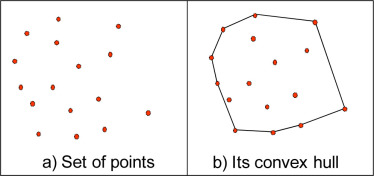
\includegraphics[width=0.8\textwidth]{Figures/convex hull.jpg}
% 	\caption{Convex Hull}
% 	\label{fig:convex hull}
% \end{figure}

\section{Synthesis of the Study}

The conducted review of related literature provides a comprehensive overview of existing methods, techniques, and technologies used for volume measurement, point cloud acquisition devices, and volume measurement using 3D point cloud data. It highlights the importance of enhancing post-harvest processing and storage technology to meet increasing global demand and minimize waste, emphasizing the role of advanced monitoring and management techniques in improving production efficiency and safety standards.

Various methods for volume measurement, including traditional level measurements and emerging technologies such as LiDAR, have been discussed. While traditional methods like weighted fiberglass tape provide a single data point, newer technologies offer more detailed and accurate measurements. Point cloud acquisition devices, particularly LiDAR, have emerged as powerful tools for generating detailed 3D models of objects or environments. Techniques for transforming 2D LiDAR scanners into 3D point cloud scanners have been explored, highlighting the use of rotating mechanisms and processing algorithms.

Additionally, the review discusses frameworks for point cloud processing, visualization, and mapping, emphasizing the importance of utilizing tools like ROS and PCL for efficient data handling. Techniques and methods for volume estimation using computational geometry, such as Delaunay triangulation and voxelization, have been examined, along with their applications in various industries.

Furthermore, the integration of Robot Web Tools (RWT) with ROS for remote monitoring of robots has been explored, demonstrating its potential in enabling real-time interaction and control of robots over the web. Several studies have demonstrated the capabilities of RWT in disaster management, cloud robotics, and real-time sensor data analysis.

Given the advancements in point cloud acquisition devices, volume measurement techniques, and web-based robotics interfaces, this study focused on integrating and utilizing these technologies and methods to provide an alternative solution to existing technology used in storage volume calculation. By leveraging existing technologies and methodologies, the aim of this study was to develop a feasible approach for enhancing storage technology especially in volume measurement technology.

\begin{landscape}
	\begin{table}[h]
		\begin{threeparttable}
			\caption{Research Synthesis Matrix}
			\label{ch2:tab:research-synthesis-matrix}
			\begin{tabular}{p{2cm}  p{4.3cm} p{4.3cm} p{4.3cm} p{4.3cm}}
				\toprule
				\textbf{\thead{Literature}}                                                                                                                                                                                                                              & \textbf{\thead{Specific Objectives}} & \textbf{\thead{Methodology}} & \textbf{\thead{Problem: \\ Unknown/Gap}} & \textbf{\thead{Remarks}}                                                                                                                                                \\ \midrule
				\citet{kang2018}                                                                                                                                                                                                                                         &
				To reconstruct complex 3D models using a low-cost 2D LiDAR by integrating an external rotary mechanism. The study sought to evaluate the feasibility and performance of this method in acquiring accurate 3D point cloud data.                           &
				The study used a 2D low-cost off-the-shelf LiDAR sensor combined with an external rotary mechanism to achieve 3D reconstruction. Experimental tests were conducted to assess the accuracy and effectiveness of this setup in 3D point cloud acquisition. &
				The research addressed the challenge of using low-cost 2D LiDAR sensors for 3D reconstruction, focusing on the increased complexity in hardware or software required for accurate 3D point cloud acquisition.                                            &
				Concluded that integrating an external rotary mechanism allows low-cost 2D LiDAR sensors to perform 3D point cloud acquisition effectively. This approach increases system complexity but provides a cost-effective solution for 3D model reconstruction.
				\\ \midrule

				\citet{yuan2021}                                                                                                                                                                                                                                         &
				Aimed to create a 3D point cloud representation of the environment using a 2D LiDAR rotated by a stepper motor. The study focused on minimizing                                                                                                          &
				The methodology involved rotating a 2D LiDAR using a stepper motor with the initial motor shaft position defined by photoelectric switches and                                                                                                           &
				The research tackled the challenge of synchronizing a 2D LiDAR with a stepper motor for 3D point cloud creation without an absolute angle                                                                                                                &
				Demonstrated that a 2D LiDAR, when rotated by a stepper motor and properly calibrated, can effectively generate a 3D point                                                                                                                                                                                                                               \\
				\midrule
			\end{tabular}
		\end{threeparttable}
	\end{table}
\end{landscape}

\newpage

\begin{landscape}
	\begin{table*}[ht]
		\begin{threeparttable}
			\caption*{\textbf{Table \ref{ch2:tab:research-synthesis-matrix}} (contd.)}
			\label{ch2:tab:research-synthesis-matrix-contd.}
			\begin{tabular}{p{2cm}  p{4.3cm} p{4.3cm} p{4.3cm} p{4.3cm}}
				\midrule
				{}                                                                                                                                                                                                                               &
				costs by employing a stepper motor and ensuring accurate system calibration to address errors from the lack of an absolute angle position.                                                                                       &
				shading sheets. Intensive calibration was conducted to correct system errors by synchronizing the 2D LiDAR with the stepper motor, ensuring accurate 3D point cloud acquisition.                                                 &
				position. The focus was on developing a cost-effective yet precise solution for 3D data acquisition.                                                                                                                             &
				representation. The use of photoelectric switches and shading sheets for initial position definition and intensive calibration ensures system accuracy, providing a low-cost solution for 3D environment modeling.                     \\
				\midrule
				\citet{clar2022}                                                                                                                                                                                                                 &
				Aimed to develop a more accurate and efficient method for estimating the volume of raw materials in silos using 3D mapping with point cloud processing.                                                                          &
				The study used a 2D LiDAR scanner to scan a prototype silo, processed the data with ROS, and converted 2D scans to 3D using an algorithm. Outliers were removed statistically, and the Convex Hull method calculated the volume. &
				The research addressed the challenge of accurately estimating silo volumes due to uneven surfaces, which conventional methods struggle with. It highlighted the need for a more precise, efficient, and scalable solution.       &
				Showed that the proposed method significantly improved volume estimation accuracy, however, The study conducted in a laboratory test and needs for large scale and a more compact and portable solution for larger-scale applications. \\
				\midrule
			\end{tabular}
		\end{threeparttable}
	\end{table*}
\end{landscape}

\newpage

\begin{landscape}
	\begin{table*}[ht]
		\begin{threeparttable}
			\caption*{\textbf{Table \ref{ch2:tab:research-synthesis-matrix}} (contd.)}
			\label{ch2:tab:research-synthesis-matrix-contd.}
			\begin{tabular}{p{2cm}  p{4.3cm} p{4.3cm} p{4.3cm} p{4.3cm}}
				\midrule
				\citet{kim2002}                                                                                                                                                                                                        &
				Aimed to explore and address the convex hull problem in computational geometry, focusing on developing efficient algorithms for its computation.                                                                       &
				Utilized various techniques, including the Voronoi diagram, Delaunay triangulation, furthest-site Voronoi diagram, furthest-site Delaunay triangulation, and half-space intersection around a point.                   &
				The research addressed the challenges of accurately computing convex hulls in high-dimensional spaces and resolving issues related to round-off errors in floating-point calculations.                                 &
				The studies demonstrated that the Qhull program is effective in computing convex hulls, calculating volumes, surface areas, and providing convex hull approximations.                                                    \\
				\midrule
				\citet{jeong2018}                                                                                                                                                                                                      &
				Aimed to develop an explicit hybrid numerical methodology for 3D volume reconstruction from unorganized point clouds, utilizing a modified Allen-Cahn equation and a 3D binary picture segmentation method.            &
				The study introduced a novel technique combining the modified Allen-Cahn equation with 3D binary picture segmentation for reconstructing 3D volumes from unorganized point clouds.                                     &
				The research addressed the challenge of efficiently reconstructing 3D volumes, a process essential for various practical applications but often hampered by inefficiencies and lack of robustness in existing methods. &
				Demonstrated that the proposed hybrid numerical methodology is both efficient and resilient, making it highly suitable for practical applications like 3D model printing from scanned data.                              \\
				\midrule
			\end{tabular}
		\end{threeparttable}
	\end{table*}
\end{landscape}